\documentclass[conference]{IEEEtran}
% \documentclass[conference,compsoc]{IEEEtran}
%\usepackage[includefoot,includehead,a4paper,top=1.5cm,bottom=1.5cm,left=2cm,right=2cm]{geometry}
%\usepackage{fancyhdr}
\usepackage[usenames,dvipsnames]{color}  % see http://en.wikibooks.org/wiki/LaTeX/Colors
%\usepackage{titlesec}
\usepackage[latin1]{inputenc}
%\usepackage{hyperref}
\usepackage[pdfborder={0 0 0},colorlinks=true,urlcolor=ForestGreen,linkcolor=black,citecolor=ForestGreen,bookmarks=true]{hyperref}
%\usepackage[pdfborder={0 0 0},colorlinks=true,urlcolor=ForestGreen,linkcolor=black,citecolor=ForestGreen,bookmarks=true,pdftitle={\doctitle},pdfauthor={\docauthor}]{hyperref}
\usepackage[labelfont=bf]{caption}
\usepackage{enumerate}

\usepackage{graphicx}
\usepackage{amsmath}
\usepackage{amssymb}
% \usepackage{url}
\usepackage{mathtools}
\usepackage{xspace}
\usepackage{multirow}
\usepackage{booktabs}
\usepackage{algorithmic}
\usepackage{algorithm}
\usepackage{xfrac}
\usepackage{fancyvrb}
\usepackage{balance}

\usepackage[british]{babel}
%\usepackage[none]{hyphenat}
%\sloppy

%\usepackage{parskip}

%\usepackage{times}
%\usepackage{palatino}     % changes the default sans serif font
%\usepackage{inconsolata}  % changes the default typewriter font

%\renewcommand{\ttdefault}{pcr}

%\edef\oldtt{\ttdefault}
%\usepackage[scaled]{beramono}
%\usepackage[T1]{fontenc}
%\renewcommand*\ttdefault{\oldtt}
%\newcommand{\bera}[1]{{\fontfamily{fvm}\selectfont #1}}

% disable ligatures such as "fi" being joined into one symbol
%\usepackage{microtype}
%\DisableLigatures[f]{encoding = *, family = * }

\graphicspath{{./}{./figures/}}

\DeclareMathOperator*{\argmin}{argmin}

\def\Vec#1{{\boldsymbol{#1}}}
\def\Mat#1{{\boldsymbol{#1}}}
\def\TODO#1{{\color{red}{\bf [TODO:} {\it{#1}}{\bf ]}}}
\def\NOTE#1{{\bf [NOTE:} {\it\color{blue}{#1}}{\bf ]}.}
\def\CHK#1{{\bf [CHECK:} {\it\color{red} {#1}}{\bf ]}.}
\def\eg{eg.\xspace}
\def\ie{ie.\xspace}
\def\etal{et~al.\xspace}

%\renewcommand{\baselinestretch}{1.1}\small\normalsize

%\setlength{\parindent}{0ex}
%\setlength{\parskip}{2ex plus1ex minus1ex}
%\setlength{\parskip}{2ex}

\title{\LARGE\bf An Open Source C++ Implementation of Multi-Threaded\\Gaussian~Mixture~Models, k-Means and Expectation Maximisation}
\author
  {
  Conrad Sanderson~{$^{\dagger\diamond}$} and Ryan Curtin~{$^{\ddagger}$}\\
  ~\\
  {$^\dagger$}  Data61, CSIRO, Australia\\
  {$^\ddagger$} Symantec Corporation, USA\\
  {$^\diamond$} University of Queensland, Australia\\
  %{$^\ast$}     Arroyo Consortium
  }

%\begin{small}
%{$^\dagger$}  Data61, CSIRO, Australia\\
%{$^\ddagger$} Symantec Corporation, USA\\
%{$^\diamond$} University of Queensland, Australia\\
%{$^\ast$}     Arroyo Consortium
%\end{small}
%\end{minipage}
%\end{center}


%\titleformat*{\section}{\bf\normalsize\large}
%\titleformat*{\subsection}{\bf\normalsize}

%\titlespacing{\section}{0pt}{\parskip}{0ex}
%\titlespacing{\subsection}{0pt}{\parskip}{0ex}
%\titlespacing{\subsubsection}{0pt}{\parskip}{0ex}

%\makeatletter
%\g@addto@macro\normalsize{%
%  \setlength\abovedisplayskip{1ex}
%  \setlength\belowdisplayskip{1ex}
%  \setlength\abovedisplayshortskip{1ex}
%  \setlength\belowdisplayshortskip{1ex}
%}
%\makeatother

\begin{document}

%\pagestyle{empty}
%\lhead{}
%\lhead{\textcolor{Green}{\small\doctitle}}
%\chead{}
%\rhead{}
%\lfoot{}
%\cfoot{}
%\cfoot{\small \thepage}
%\rfoot{}


%\centerline{\textcolor{red}{\bf[DRAFT - WORK IN PROGRESS - VERSION 2017-07-14b]}}

%\begin{center}
%{\Large\bf\doctitle}
%\end{center}

%\begin{center}

%\begin{minipage}{0.5\textwidth}
%{\large\it Conrad Sanderson~{$^{\dagger\diamond\ast}$} and Ryan Curtin~{$^{\ddagger\ast}$}}\\

%\begin{small}
%{$^\dagger$}  Data61, CSIRO, Australia\\
%{$^\ddagger$} Symantec Corporation, USA\\
%{$^\diamond$} University of Queensland, Australia\\
%{$^\ast$}     Arroyo Consortium
%\end{small}
%\end{minipage}
%\end{center}
\maketitle

\section*{Abstract}

Modelling of multivariate densities is a core component in many signal processing, pattern recognition and machine learning applications.
We provide an overview of a fast implementation of Gaussian mixture models in the C++ language,
which employs multi-threaded (parallelised) versions of the Expectation Maximisation (EM) and {\it k}-means training algorithms.
Parallelisation is achieved through reformulation of the EM and {\it k}-means algorithms into a MapReduce-like framework
and employing OpenMP compiler directives.
We demonstrate that the parallelised implementation achieves a speedup of an order of magnitude on a recent 16 core machine.
The implementation is included as a user-friendly class in recent releases of the open source Armadillo C++ linear algebra library,
which is provided under the permissive Apache 2.0 license, allowing unencumbered use in commercial products.


% \newpage
% \pagestyle{fancy}
% \lhead{}
% %\lhead{\textcolor{Green}{\small\doctitle}}
% \chead{}
% \rhead{}
% \lfoot{}
% \cfoot{}
% %\cfoot{\small \thepage}
% \rfoot{}

\section{Introduction}

Modelling multivariate data through mixtures of Gaussians, also known as Gaussian Mixture Models (GMMs),
has many uses in fields such as statistics, econometrics, pattern recognition, machine learning and computer vision.
Examples of applications include
multi-stage feature extraction for action recognition~\cite{Carvajal_2016a},
modelling of intermediate features~\cite{Ge_ICIP_2015} derived from deep convolutional neural networks~\cite{Ge_2016,LeCun_Nature_2015},
classification of human epithelial cell images~\cite{Wiliem_PR_2014},
implicit sparse coding for face recognition~\cite{Wong_2014},
and probabilistic foreground estimation for surveillance systems~\cite{Reddy_2013}.

In the GMM approach, a distribution of samples (vectors) is modelled as:
%
\begin{equation}
  p(\Vec{x} | \lambda) = \sum\nolimits_{g=1}^{N_G} w_g ~ {{\mathcal{N}}}( \Vec{x} ~|~ \Vec{\mu}_g, \Mat{\Sigma}_g )
  \label{eqn:gmm_prob}
\end{equation}%
%
where $\Vec{x}$ is a $D$-dimensional vector,
$w_g$ is the weight for component $g$ (with constraints $\sum\nolimits_{g=1}^{N_G} w_g = 1$, $w_g \geq 0$),
and
${{\mathcal{N}}}( \Vec{x} | \Vec{\mu}, \Mat{\Sigma})$ is a $D$-dimensional Gaussian density function with mean $\Vec{\mu}$ and covariance matrix $\Mat{\Sigma}$:
%
\begin{equation}
  {{\mathcal{N}}}( \Vec{x} | \Vec{\mu}, \Mat{\Sigma} )  = 
  \frac{1}{ (2\pi)^{\frac{D}{2}} | \Mat{\Sigma}|^{\frac{1}{2}} }
  \exp \left[ -\frac{1}{2} (\Vec{x}-\Vec{\mu})^\top \Mat{\Sigma}^{-1} (\Vec{x}-\Vec{\mu}) \right]
  \label{eqn:gaussian}
\end{equation}%
%
The full parameter set can be compactly stated as $\lambda = \{ w_g, \Vec{\mu}_g, \Mat{\Sigma}_g \}_{g=1}^{N_G}$,
where $N_G$ is the number of Gaussians.



TODO: choice for $\Mat{\Sigma}$: full or diagonal

TODO: mention methods for selecting  $N_G$ ?  

Choosing the optimal $N_G$ is typically data dependent and beyond the scope of this work; see~\cite{Hamerly_2003,Pelleg_2000} for example methods.

TODO: overview of all the sections

~
\section{\small Expectation Maximisation and Multi-Threading}
\label{sec:param_em}

\noindent
The overall likelihood for a set of samples, $X=\{\Vec{x}_i\}_{i=1}^{N_V}$,
is found using $p(X | \lambda) = \prod\nolimits_{i=1}^{N_V} p(\Vec{x}_i | \lambda)$.
A~parameter set $\lambda$ that suitably models the underlying distribution of $X$ can be estimated using a particular instance of the Expectation Maximisation (EM) algorithm~\cite{Dempster77, McLachlan-2008, Moon96, Redner84}.
As its name suggests, the EM algorithm is comprised of iterating two steps: the {\it expectation} step, followed by the {\it maximisation} step.
GMM parameters generated by the previous iteration~($\lambda^{\textrm{old}}$) are used
by the current iteration to generate a new set of parameters~($\lambda^{\textrm{new}}$), such that:
%
\begin{eqnarray}
	p(X|\lambda^{\textrm{new}}) \geq p(X|\lambda^{\textrm{old}})
\end{eqnarray}
%
In a direct implementation of the EM algorithm specific to GMMs,
the estimated versions of the parameters ($\widehat{w}_g$, $\widehat{\Vec{\mu}}_g$, $\widehat{\Mat{\Sigma}}_g$)
within one iteration are calculated as follows:
%
\begin{eqnarray}
  l_{g,i}                  & = & \frac{w_g ~ {{\mathcal{N}}}( \Vec{x}_i | \Vec{\mu}_g, \Mat{\Sigma}_g )}{\sum\nolimits_{k=1}^{N_G} w_k ~ {{\mathcal{N}}}( \Vec{x}_i | \Vec{\mu}_k, \Mat{\Sigma}_k )}, \label{eqn:aposteriori} \\
  L_g                      & = & \sum\nolimits_{i=1}^{N_V} l_{g,i}, \label{eqn:em_sum_lhood} \\
  \widehat{w}_g            & = & \frac{L_g}{N_V},  \label{eqn:em_weight} \\
  \widehat{\Vec{\mu}}_g    & = & \frac{1}{L_g} \sum\nolimits_{i=1}^{N_V} \Vec{x}_i ~ l_{g,i}  \label{eqn:em_mean}, \\
  \widehat{\Mat{\Sigma}}_g & = & \frac{1}{L_g} \sum\nolimits_{i=1}^{N_V} (\Vec{x}_i - \widehat{\Vec{\mu}}_g)(\Vec{x}_i - \widehat{\Vec{\mu}}_g)^\top l_{g,i}. \label{eqn:em_cov}
%                           & = &  \frac{1}{L_g} \left[ \sum\nolimits_{i=1}^{N_V} \Vec{x}_i \Vec{x}_i^\top l_{g,i} \right] - \widehat{\Vec{\mu}}_g \widehat{\Vec{\mu}}_g^\top.
\end{eqnarray}

\noindent
Once the estimated parameters for all Gaussians are found, the parameters are updated:

\begin{equation}
\left\{ w_g, \Vec{\mu}_g, \Mat{\Sigma}_g \right\}_{g=1}^{N_G} = \left\{ \widehat{w}_g, \widehat{\Vec{\mu}}_g, \widehat{\Mat{\Sigma}}_g \right\}_{g=1}^{N_G}
\end{equation}

\noindent and the iteration starts anew.
The process is typically repeated until the number of iterations has reached a pre-defined number,
and/or the increase in the overall likelihood after each iteration falls below a pre-defined threshold.

In Eqn.~(\ref{eqn:aposteriori}), $l_{g,i} \in [0,1]$ is the {a-posteriori} probability of Gaussian $g$ given $\Vec{x}_i$ and current parameters.
Thus the estimates $\widehat{\Vec{\mu}}_g$ and $\widehat{\Mat{\Sigma}}_g$ are weighted versions of the
sample mean and sample covariance, respectively.

Overall, the algorithm is a hill climbing procedure for maximising $p(X | \lambda)$.
While there are no guarantees that it will reach a global maximum, it is guaranteed to monotonically converge to a saddle point or a local maximum~\cite{Dempster77,Duda01,Mitchell97}.
The above implementation can also be interpreted as an unsupervised probabilistic clustering procedure,
with $N_G$ being the assumed number of clusters.
For a full derivation of the EM algorithm tailored to GMMs, the reader is directed to~\cite{Bilmes98,Redner84}. % or Appendix~A. %~\ref{app:em_algorithm}.


\subsection{Reformulation for Parallel Execution}
\label{sec:param_em_parallel}

The EM algorithm is quite computationally intensive.
This is in large part due to the use of the $\exp(\cdot)$ function, which needs to be applied numerous times for each and every sample.
Fortunately, multi-core (multi-threaded) machines are now quite common and accessible, allowing for parallel execution.

One approach for parallelisation is the MapReduce framework~\cite{MapReduce_2004},
where data is split into chunks and farmed out to worker threads for processing (mapping).
The results are then collected and combined (reduced) to produce the final result.
Below we provide a reformulation of the EM algorithm into a MapReduce-like framework.

As Eqn.~(\ref{eqn:aposteriori}) can be executed independently for each sample,
the summations in Eqns.~(\ref{eqn:em_sum_lhood}) and (\ref{eqn:em_mean}) can be split into separate sets of summations,
where the summation in each set can be executed independently and in parallel with other sets.
To allow similar splitting of the summation for calculating covariance matrices,
Eqn.~(\ref{eqn:em_cov}) needs to be rewritten into the following form:
%
\begin{equation}
  \widehat{\Mat{\Sigma}}_g = \frac{1}{L_g} \left[ \sum\nolimits_{i=1}^{N_V} \Vec{x}_i \Vec{x}_i^\top l_{g,i} \right] - \widehat{\Vec{\mu}}_g \widehat{\Vec{\mu}}_g^\top.
\end{equation}

The multi-threaded estimation of the parameters can now be formally stated as follows.
Given $N_T$ threads, the training samples are split into $N_T$ chunks, with each chunk containing approximately the same amount of samples.
For thread with index $t \in [1,N_T]$, the start index of the samples is denoted by $i^{[t]}_{\textrm{start}}$,
while the end index is denoted by $i^{[t]}_{\textrm{end}}$.
For~each thread $t$ and Gaussian $g \in [1,N_G]$, accumulators $\widetilde{L}_g^{[t]}$, $\widetilde{\Vec{\mu}}_g^{[t]}$ and $\widetilde{\Mat{\Sigma}}_g^{[t]}$
are calculated as follows:
%
\begin{eqnarray}
  %\mbox{for} ~~ g = 1, \cdots, N_g:  \nonumber \\
  %
  \widetilde{L}_g^{[t]}            & = & \sum\nolimits_{j = i^{[t]}_{\textrm{start}}}^{i^{[t]}_{\textrm{end}}} l_{g,j},                             \\ % acc_norm_lhoods
  \widetilde{\Vec{\mu}}_g^{[t]}    & = & \sum\nolimits_{j = i^{[t]}_{\textrm{start}}}^{i^{[t]}_{\textrm{end}}} l_{g,j} ~ \Vec{x}_j,                 \\ % acc_mean
  %\widetilde{\Mat{\Sigma}}_g^{[t]} & = & \sum\nolimits_{j = i^{[t]}_{\textrm{start}}}^{i^{[t]}_{\textrm{end}}} l_{g,j} ~ \Vec{x}_j \odot \Vec{x}_j    % acc_dcov
  \widetilde{\Mat{\Sigma}}_g^{[t]} & = & \sum\nolimits_{j = i^{[t]}_{\textrm{start}}}^{i^{[t]}_{\textrm{end}}} l_{g,j} ~ \Vec{x}_j \Vec{x}_j^\top.    % acc_dcov
\end{eqnarray}%
%
where $l_{g,j}$ is defined in Eqn.~(\ref{eqn:aposteriori}).
%while $\odot$ represents the Schur product (element-wise multiplication).

Once the accumulators for all threads are calculated,
for each Gaussian $g$ the reduction operation combines them to form the estimates of $\widehat{w}_g$, $\widehat{\Vec{\mu}}_g$ and $\widehat{\Mat{\Sigma}}_g$ as follows:
%
\begin{eqnarray}
  L_g                      & = & \sum\nolimits_{t=1}^{N_T} \widetilde{L}_g^{[t]},                           \\ % acc_norm_lhood
  \widehat{w}_g            & = & \frac{L_g}{N_V},                                                           \\
  \widehat{\Vec{\mu}}_g    & = & \frac{1}{L_g} \sum\nolimits_{t=1}^{N_T} \widetilde{\Vec{\mu}}_g^{[t]},     \\
  \widehat{\Mat{\Sigma}}_g & = & \frac{1}{L_g} \sum\nolimits_{t=1}^{N_T} \widetilde{\Mat{\Sigma}}_g^{[t]} - \widehat{\Vec{\mu}}_g \widehat{\Vec{\mu}}_g^\top.
\end{eqnarray}

~

\subsection{Improving Numerical Stability}

Due to the necessarily limited precision of numerical floating point representations~\cite{Goldberg_1991,Monniaux_2008},
the direct computation of Eqns.~(\ref{eqn:gmm_prob}) and (\ref{eqn:gaussian}) can quickly lead to numerical underflows or overflows.
%To address this problem, the logarithm version of Eqn.~(\ref{eqn:gmm_prob}) can be used:
To address this problem, the logarithm version of Eqn.~(\ref{eqn:gaussian}) can be used:
%
\begin{multline}
  \log {{\mathcal{N}}}( \Vec{x} | \Vec{\mu}, \Mat{\Sigma} )
%   & = &
%   \log \left\{
%   \frac{1}{ (2\pi)^{\frac{D}{2}} | \Mat{\Sigma}|^{\frac{1}{2}} }
%   \exp \left[ -\frac{1}{2} (\Vec{x}-\Vec{\mu})^\top \Mat{\Sigma}^{-1} (\Vec{x}-\Vec{\mu}) \right]
%   \right\} \\
% %
%   & = &
%   \log \left\{
%   \frac{1}{ (2\pi)^{\frac{D}{2}} | \Mat{\Sigma}|^{\frac{1}{2}} } \right\}
%   + 
%   \log \left\{
%   \exp \left[ -\frac{1}{2} (\Vec{x}-\Vec{\mu})^\top \Mat{\Sigma}^{-1} (\Vec{x}-\Vec{\mu}) \right]
%   \right\} \\
% %
%   & = &
%   -  \log \left\{
%   (2\pi)^{\frac{D}{2}} | \Mat{\Sigma}|^{\frac{1}{2}} \right\}
%   + 
%   -\frac{1}{2} (\Vec{x}-\Vec{\mu})^\top \Mat{\Sigma}^{-1} (\Vec{x}-\Vec{\mu})
%   \\ 
% %
%   & = &
%   - \left(
%   \log \left\{ (2\pi)^{\frac{D}{2}} \right\} + \log \left\{  | \Mat{\Sigma}|^{\frac{1}{2}} \right\}
%   \right)
%   + 
%   -\frac{1}{2} (\Vec{x}-\Vec{\mu})^\top \Mat{\Sigma}^{-1} (\Vec{x}-\Vec{\mu})
%   \\
% %
%   & = &
%   - \left(
%   \frac{D}{2} \log \left( 2\pi \right)
%   +
%   \frac{1}{2} \log ( |\Mat{\Sigma}| )
%   \right)
%   -
%   \frac{1}{2} (\Vec{x}-\Vec{\mu})^\top \Mat{\Sigma}^{-1} (\Vec{x}-\Vec{\mu})
%   \\
% %
  = -\left\{\sfrac{D}{2} \log \left( 2\pi \right)
  +
  \sfrac{1}{2} ~ \log ( |\Mat{\Sigma}| )
  \right\} \\ - \sfrac{1}{2} (\Vec{x}-\Vec{\mu})^\top \Mat{\Sigma}^{-1} (\Vec{x}-\Vec{\mu}).
\end{multline}

The corresponding logarithm version of Eqn.~(\ref{eqn:gmm_prob}) is:
%
\begin{multline}
\log \sum\nolimits_{g=1}^{N_G} w_g ~ {{\mathcal{N}}}( \Vec{x} ~|~ \Vec{\mu}_g, \Mat{\Sigma}_g )
 = \\
 \log \sum\nolimits_{g=1}^{N_G} \exp\left[ \log \left\{ w_g {{\mathcal{N}}}( \Vec{x} ~|~ \Vec{\mu}_g, \Mat{\Sigma}_g ) \right\} \right].
\label{eqn:log_gmm}
\end{multline}

\noindent
The right hand side of Eqn.~(\ref{eqn:log_gmm}) can be expressed as a repeated addition in the form of:
%
\begin{equation}
\log\left( \exp\left[\log(a)\right] + \exp\left[\log(b)\right] \right),
\end{equation}%
%
which in turn can be rewritten in the form of:
%
\begin{equation}
\log(a) + \log\left( 1 + \exp\left[ \log(b) - \log(a) \right] \right).
\end{equation}%

\noindent
In the latter form, if we ensure that {$\log(a) \geq \log(b)$} (through swapping $\log(a)$ and $\log(b)$ when required),
the exponential will always produce values $\leq 1$ which helps to reduce the occurrence of overflows.

% Formally, the robust version of \mbox{\small $\log(\exp\left[\log(a)\right] + \exp\left[\log(b)\right])$} can be expressed as 
% $\operatorname{\Psi}(\log(a), \log(b))$ is used as 
% %
% \begin{eqnarray}
% \operatorname{\Psi}(\log(a), \log(b))
% & = & \left\{
% \begin{array}{ll}
% \operatorname{\Omega}(\log(a),\log(b)), & \mbox{if} ~ \log(a) \geq \log(b) \\
% \operatorname{\Omega}(\log(b),\log(a)), & \mbox{otherwise}
% \end{array}
% \right. \nonumber \\
% %
% \operatorname{\Omega}(\log(a), \log(b))
% & = & \left\{
% \begin{array}{ll}
% \log(a),                   & \mbox{if} ~ (\log(b)-\log(a)) < \operatorname{log\_floor} \mbox{~or~} (\log(b)-\log(a)) \notin \mathbb{R} \\
% \log(a) + \log(1 + \exp(\log(b)-\log(a))),  & \mbox{otherwise} 
% \end{array}
% \right.  \nonumber
% \end{eqnarray}
% %
% In the above,
% $\operatorname{log\_floor}$ is a machine dependent constant, equal to approximately
% $\log(10^{-323})$ when using double precision floating point values%
% \footnote
%   {
%   The exact value in the C++ implementation is equal to {\it log({std::numeric\_limits{\textless}T{\textgreater}::min()})},
%   where {\it T} represents a floating point type (ie., either {\it float} or {\it double}).
%   }%
% .


% Given the logarithm versions of Eqns.~(\ref{eqn:gmm_prob}) and (\ref{eqn:gaussian}),
% the logarithm version of Eqn.~(\ref{eqn:aposteriori}) can be expressed as:



\section{Initial Parameter Estimation via {\it k}-Means}
\label{sec:param_km}

As a starting point, the initial means can be set to randomly selected training vectors,
the initial covariance matrices can be set equal to identity matrices, 
and the initial weights can be uniform.
However, in a computational implementation, the $\exp()$ function as well as the matrix inverse in Eqn.~(\ref{eqn:gaussian}) are typically quite time consuming.
In order to speed up training, the initial estimate of $\lambda$ is typically provided via the {\it k}-means clustering algorithm~\cite{Bishop_2006,Duda01,Kulis_2012}
which avoids such time consuming operations.

The baseline {\it k}-means clustering algorithm is a simple iterative procedure comprised of two steps:
(i)~calculating the distance from each vector to each each mean,
and
(ii)~calculating the new version of each mean as the average of vectors which were found to be the closest to the previous version of the corresponding mean.


The $k$-means algorithm can be interpreted as a simplified version (or special case) of the EM algorithm for GMMs~\cite{Kulis_2012}.
Instead of each vector being assigned a set probabilities representing cluster membership (soft assignment),
each vector is assigned to only one cluster (hard assignment).
Furthermore, it can be assumed that the covariance matrix of each Gaussian is non-informative, diagonal, and/or shared across all Gaussians.

More formally, the estimation of model parameters is as per Eqns.~(\ref{eqn:em_weight}), (\ref{eqn:em_mean}) and (\ref{eqn:em_cov}), 
but $l_{g,i}$ is redefined~as:%
%
\begin{equation}
  l_{g,i} = \left\{
  \begin{array}{ll}
  1, & \mbox{if} ~ g = \argmin\limits_{k=1, \cdots, N_G} \operatorname{dist}(\Vec{\mu}_k, \Vec{x}_i) \\
  0, & \mbox{otherwise}
  \end{array}
  \right.
\end{equation}
%
where {$\operatorname{dist}(\Vec{a}, \Vec{b})$} is a distance metric,
such as the squared Euclidean distance: \mbox{$\operatorname{dist}(\Vec{a}, \Vec{b}) = \| \Vec{a} - \Vec{b} \|^{2}_{2}$}.

There is a potential downside to using the Euclidean distance.
When one of the dimensions within the data has a much larger range than the other dimensions,
it will dominate the contribution to the distance result, with the other dimensions effectively ignored.
To address this, it is possible to use the squared Mahalanobis distance~\cite{Bishop_2006,Duda01},
\mbox{$\operatorname{dist}(\Vec{a}, \Vec{b}) = (\Vec{a} - \Vec{b})^\top \Mat{\Sigma}^{-1}_{\mathrm{global}} (\Vec{a} - \Vec{b})$},
where $\Mat{\Sigma}_{\mathrm{global}}$ is a global covariance matrix, estimated from all available training data.
To maintain efficiency, $\Mat{\Sigma}_{\mathrm{global}}$ is typically diagonal,
which makes calculating its inverse straightforward (ie., reciprocals of the values on the main diagonal).

It is possible to implement the $k$-means algorithm is a multitude of ways,
such as the cluster splitting LBG algorithm~\cite{Linde80},
or use an elaborate strategy for selecting the initial means~\cite{Arthur_2007}.
There are also alternative implementations offering faster convergence~\cite{Elkan_2003}.

The vast majority of the computational effort for training GMMs is typically taken up by the full EM algorithm (as described in Section~\ref{sec:param_em}),
hence the speed of the {\it k}-means algorithm is not critical in the context of GMMs.
However, as the {\it k}-means algorithm is essentially a simplified version of EM,
it can be parallelised in the same way as per Section~\ref{sec:param_em_parallel}.

% \subsection{Addressing Corner Cases}

In practice it is possible that while iterating at least one of the means has no vectors assigned to it,
becoming a ``dead'' mean.
This might stem from an unfortunate starting point, 
or specifying a large value for $N_G$ for which there is an insufficient number of training samples.
As such, an additional heuristic is required to attempt to resolve this situation.
One example of resurrecting a ``dead'' mean is to make it equal to one of the vectors
that has been assigned to the most ``popular'' mean,
where the most ``popular'' mean is the mean that currently has the most vectors assigned to it.



% The pseudo-code for a direct implementation of a baseline $k$-means algorithm is shown in Figure~\ref{fig:kmeans_pseudocode}.
% 
% \begin{figure}[!b]
% \hrule
% \vspace{0.5ex}
% \begin{small}
% \begin{tabbing}
% 01: {\bf for} $g=1, ~\cdots, ~N_G$ \\
% 02: ~~ $\Vec{\mu}_g = \Vec{x}_{ \mbox{\it randi}(1, N_V) } $ ~~~ {\small // randomly select initial means} \\
% 03: {\bf endfor} \\
% 04: {\it iteration} = $1$ \\
% 05: {\it final\_iteration} = $10$ ~~~ ~~~ ~~~ {\small // empirically chosen termination condition} \\
% 06: {\it finished} = FALSE \\
% 07: {\bf while} {\it finished} $\neq$ TRUE \\
% 08: ~~ {\bf for} $i=1, ~\cdots, ~N_V$ \\
% 09: ~~ ~~ \( y_i = {\displaystyle \arg \min_{g=1, \cdots, N_G}} \operatorname{\mbox{\it dist}}(\Vec{\mu}_g, \Vec{x}_i) \) ~~~ {\small // label each vector as belonging to its closest mean} \\
% 10: ~~ {\bf endfor} \\
% 11: ~~ {\bf for} $g=1, ~\cdots, ~N_G$ \\
% 12: ~~ ~~ $n_g = \sum\nolimits_{i=1}^{N_V} \delta(y_i, g) $  ~~~ ~~~ ~~~ ~~~ ~ {\small // count the number of vectors assigned to each mean} \\
% 13: ~~ ~~ $\widehat{\Vec{\mu}}_g = \frac{1}{n_g} \sum\nolimits_{i=1}^{N_V} \Vec{x}_i \delta(y_i, g) $ ~~~ ~~~ {\small // find the new mean using vectors assigned to the old mean} \\
% 14: ~~ {\bf endfor} \\
% 15: ~~ {\it same} = TRUE \\
% 16: ~~ {\bf for} $g=1, ~\cdots, ~N_G$ \\
% 17: ~~ ~~ {\bf if} $\widehat{\Vec{\mu}}_g \neq \Vec{\mu}_g $  ~~~ ~~~ ~~~ ~~~ ~~~ ~~~ ~~~~ {\small // see if the means have changed since the last iteration} \\
% 18: ~~ ~~ ~~ {\it same} = FALSE \\
% 19: ~~ ~~ {\bf endif} \\
% 20: ~~ {\bf endfor} \\
% 21: ~~ {\bf for} $g=1, ~\cdots, ~N_G$ \\
% 22: ~~ ~~ $\Vec{\mu}_g = \widehat{\Vec{\mu}}_g$ ~~~ {\small // update the mean vectors} \\
% 23: ~~ {\bf endfor} \\
% 24: ~~ {\it iteration} = {\it iteration} + 1 \\
% 25: ~~ {\bf if} ({\it same} == TRUE) {\bf or} ({\it iteration} $>$ {\it final\_iteration})  \\
% 26: ~~ ~~ {\it finished} = TRUE \\
% 27: ~~ {\bf endif} \\
% 28: {\bf endwhile}
% \end{tabbing}
% \end{small}
% \vspace{-1ex}
% \hrule
% \caption
%   {
%   \small
%   \TODO{change to normal equations}.
%   Pseudo-code for a direct implementation of the classic $k$-means algorithm.
%   Each training vector is denoted as $\Vec{x}_i$, where $i = 1, \cdots, N_V$, with $N_V$ indicating the number of vectors available for training.
%   Each mean vector is denoted as $\Vec{\mu}_g$, where $g = 1, \cdots, N_G$, with $N_G$ indicating the number of required means (centroids).
%   The~{\it randi}$(min,max)$ function generates a uniformly distributed random integer value in the $[min,max]$ interval.
%   The~{\it dist}$(\Vec{x},\Vec{y})$ function calculates a distance between vectors $\Vec{x}$ and $\Vec{y}$, with a distance of zero indicating that the vectors are equal.
%   The~$\delta(\cdot,\cdot)$ function (Kronecker delta) is equal to either $1$ or $0$, corresponding to its two arguments either matching or not matching.
%   }
% \label{fig:kmeans_pseudocode}
% \end{figure}

% Once the estimated means $\{ \Vec{\mu}_g \}_{g=1}^{N_G}$ have been found,
% the initial weights $\{ w_g \}_{g=1}^{N_G}$ and initial covariance matrices $\{ {\Mat{\Sigma}_g} \}_{g=1}^{N_G}$
% are estimated as follows:
% %
% \begin{eqnarray}
% w_g & = & \frac{n_g}{N_V} \\
% {\mbox {\boldmath $\Sigma$}_g} & = & \frac{1}{n_g} \sum\nolimits_{i=1}^{N_V} (\Vec{x}_i - \Vec{\mu}_g)(\Vec{x}_i - \Vec{\mu}_g)^T \delta(y_i, g)
% \label{eqn:k-means_cov}
% \end{eqnarray}
% %
% \noindent
% where $n_g$ is defined on line 12 of the pseudo-code and $y_i$ on line 9.

\section{Numerical Implementation in C++}

We have provided a numerical implementation of Gaussian Mixture Models in the C++ language
as part of recent releases of the open source Armadillo C++ linear algebra library~\cite{Armadillo_JOSS_2016,Armadillo_PASC_2017}.
The library can be obtained from \href{http://arma.sourceforge.net}{http://arma.sourceforge.net}.
The implementation contains multi-threaded versions of the Expectation Maximisation (EM) and {\it k}-means training algorithms
(as overviewed in Sections~\ref{sec:param_em} and~\ref{sec:param_km}),
which can considerably speed up training.
% Parallelisation is achieved through refactoring the original EM and {\it k}-means algorithms
% into a MapReduce-like framework~\cite{MapReduce_2004} and employing OpenMP compiler directives~\cite{OpenMP_2007}.

\subsection{Achievable Speedup}

To demonstrate the achievable speedup with the multi-threaded versions of the training algorithms,
we trained a GMM with 100 Gaussians on a recent 16 core machine using synthetic data comprising 1,000,000 samples with 100 dimensions.
10 iterations of the {\it k}-means algorithm and 10 iterations of the EM algorithm were used.
The samples were stored in double precision floating point format, resulting in a total data size of approximately 762~Mb.

Figure~\ref{fig:speedup} shows that a speedup of an order of magnitude is achieved when all 16 cores are used.
We note that the actual speedup is below the idealised linear speedup,
due to memory access contention (stemming from concurrent access to memory by mulitple cores)
as well as overheads related to OpenMP and reduction operations (Section~\ref{sec:param_em_parallel}).


\begin{figure}[!b]
\centering
\begin{minipage}{1\columnwidth}
  \centering
  \begin{minipage}{0.5\textwidth}
    \centering
    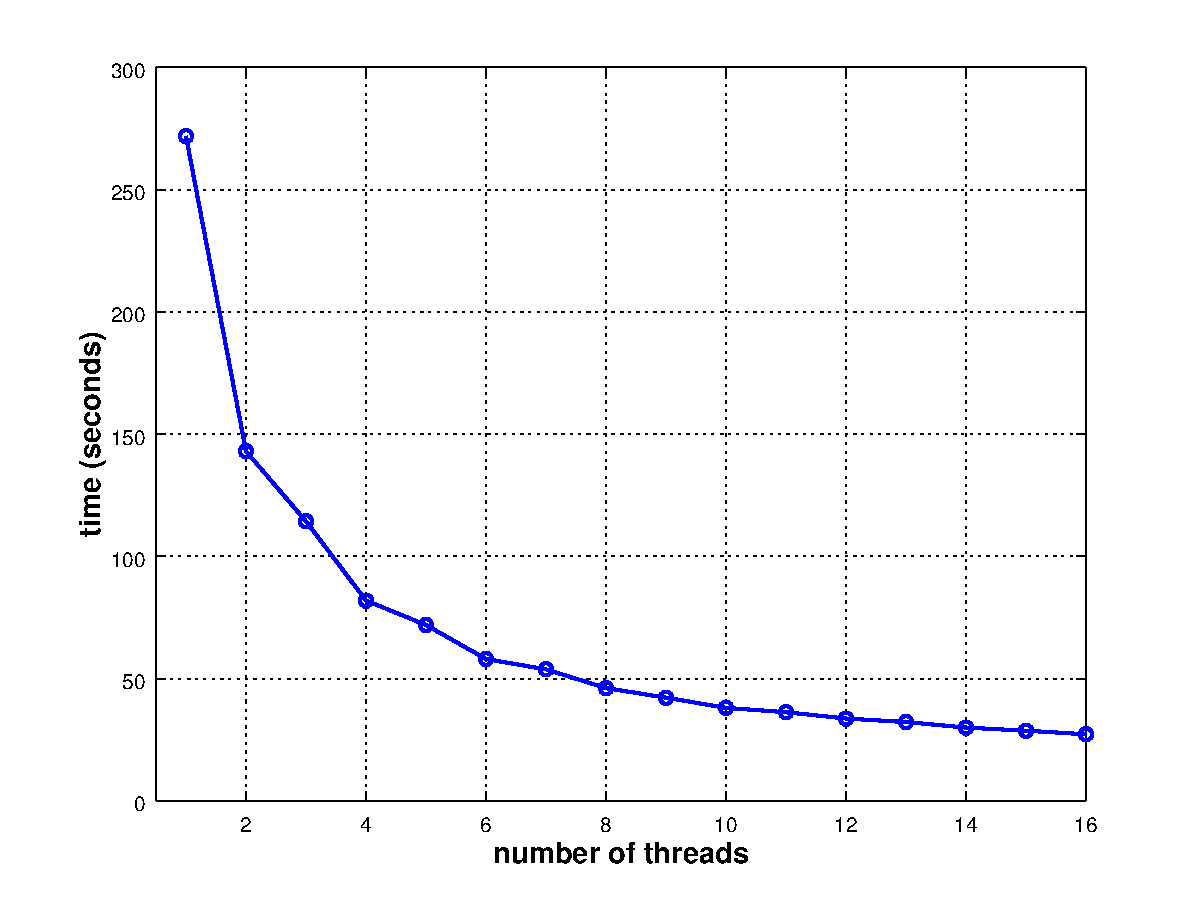
\includegraphics[width=1.1\textwidth]{plot1.pdf}\\
    {(a)}
  \end{minipage}%
  \begin{minipage}{0.5\textwidth}
    \centering
    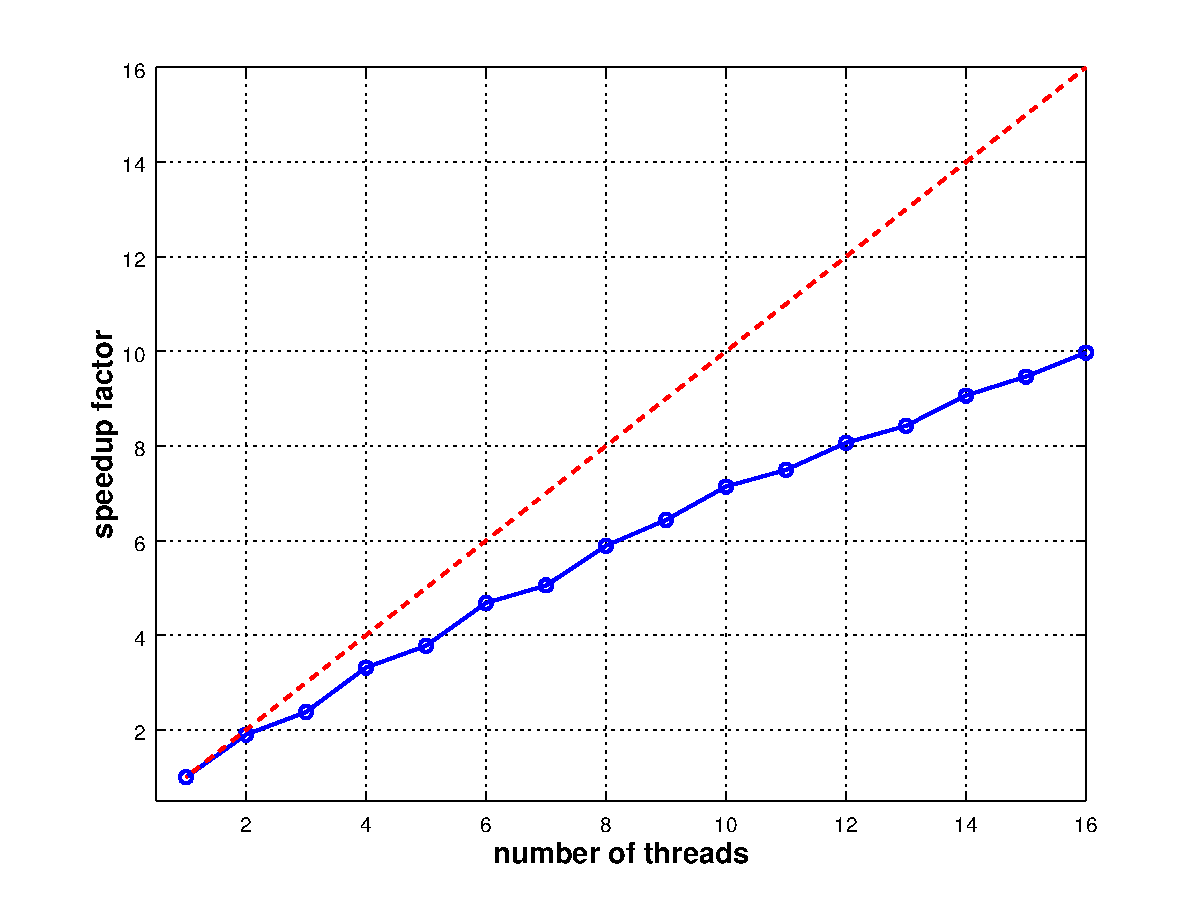
\includegraphics[width=1.1\textwidth]{plot2.pdf}\\
    {(b)}
  \end{minipage}
\end{minipage}
\caption
  {
  Execution characteristics for training a 100 component GMM
  to model synthetic data comprising 1,000,000 samples with 100 dimensions
  using 10 iterations of the {\it k}-means algorithm and 10 iterations of the EM algorithm:
  {\bf (a)}~total time taken depending on the number of threads;
  {\bf (b)}~corresponding speedup factor compared to using one thread (blue line), and idealised linear speedup under the assumption of no overheads and no memory access contention (red dotted line).
  The modelling was done on a machine with dual Intel Xeon E5-2620~v4 CPUs, providing 16 independent processing cores.
  Compilation was done with GCC 5.4 using the following switches: \texttt{-O3 -march=native -fopenmp}.
  }
\label{fig:speedup}
\end{figure}

\subsection{User Accessible Classes and Functions}

The implementation is provided as two user accessible classes within the {\it arma} namespace:
{\it gmm\_diag} and {\it fgmm\_diag}.
The former uses double precision floating point values, while the latter uses single precision floating point values.
For an instance of the double precision {\it gmm\_diag} class named as {\bf M},
its member functions and variables are listed below.
Figure~\ref{fig:example_usage} contains a complete C++ program which demonstrates usage of the {\it gmm\_diag} class.

In the description below, all vectors and matrices refer to corresponding objects from the Armadillo library;
scalars have the type {\it double},
matrices have the type {\it mat},
column vectors have the type {\it vec},
row vectors have the type {\it rowvec},
row vectors of unsigned integers have the type {\it urowvec},
and indices have the type {\it uword} (representing an unsigned integer).
When using the single precision {\it fgmm\_diag} class,
all vector and matrix types have the {\it f} prefix (for example, {\it fmat}),
while scalars have the type {\it float}.
The word ``heft'' is explicitly used in the classes as a shorter version of ``weight'', while keeping the same meaning with the context of GMMs.

\begin{small}
\begin{itemize}

\item
{\bf M.log\_p(V)}\\
return a scalar (double precision floating point value) representing the log-likelihood of column vector {\bf V}

\item
{\bf M.log\_p(V, g)}\\
return a scalar (double precision floating point value) representing the log-likelihood of column vector {\bf V},
according to Gaussian with index {\bf g} (specified as an unsigned integer of type {\it uword})

\item
{\bf M.log\_p(X)}\\
return a row vector (of type {\it rowvec}) containing log-likelihoods of each column vector in matrix {\bf X}


\item
{\bf M.log\_p(X, g)}\\
return a row vector containing log-likelihoods of each column vector in matrix {\bf X},
according to Gaussian with index {\bf g}  (specified as an unsigned integer of type {\it uword})

\item
{\bf M.avg\_log\_p(X)}\\
return a scalar (double precision floating point value) representing the average log-likelihood of all column vectors in matrix {\bf X}

\item
{\bf M.avg\_log\_p(X, g)}\\
return a scalar (double precision floating point value) representing the average log-likelihood of all column vectors in matrix {\bf X},
according to Gaussian with index {\bf g}  (specified as an unsigned integer of type {\it uword})

\item
{\bf M.assign(V, dist\_mode)}\\
return an unsigned integer (of type {\it uword}) representing the index of the closest mean (or Gaussian) to vector {\bf V};\\
parameter {\bf dist\_mode} is one of:

\begin{tabular}{ll}
{\bf eucl\_dist} & Euclidean distance (takes only means into account) \\
{\bf prob\_dist} & probabilistic ``distance'', defined as the inverse likelihood\\
                 & (takes into account means, covariances and hefts)
\end{tabular}

\item
{\bf M.assign(X, dist\_mode)}\\
return a row vector of unsigned integers (of type {\it urowvec}) containing the indices of the closest means (or Gaussians) to each column vector in matrix {\bf X};
parameter {\bf dist\_mode} is either {\bf eucl\_dist} or {\bf prob\_dist}, as per the {\bf .assign()} function above

\item
{\bf M.raw\_hist(X, dist\_mode)}\\
return a row vector of unsigned integers (of type {\it urowvec}) representing the raw histogram of counts;
each entry is the number of counts corresponding to a Gaussian;
each count is the number times the corresponding Gaussian was the closest to each column vector in matrix {\bf X};
parameter {\bf dist\_mode} is either {\bf eucl\_dist} or {\bf prob\_dist}, as per the {\bf .assign()} function above

\item
{\bf M.norm\_hist(X, dist\_mode)}\\
similar to the {\bf .raw\_hist()} function above; return a row vector (of type {\it rowvec}) containing normalised counts; the vector sums to one;
parameter {\bf dist\_mode} is either {\bf eucl\_dist} or {\bf prob\_dist}, as per the {\bf .assign()} function above

\item
{\bf M.generate()}\\
return a column vector representing a random sample generated according to the model's parameters

\item
{\bf M.generate(N)}\\
return a matrix containing {\bf N} column vectors, with each vector representing a random sample generated according to the model's parameters

\item
{\bf M.save(filename)}\\
save the model to a file

\item
{\bf M.load(filename)}\\
load the model from a file

\item
{\bf M.n\_gaus()}\\
return an unsigned integer (of type {\it uword}) containing the number of means/Gaussians in the model

\item
{\bf M.n\_dims()}\\
return an unsigned integer (of type {\it uword}) containing the dimensionality of the means/Gaussians in the model

\item
{\bf M.reset(n\_dims, n\_gaus)}\\
set the model to have dimensionality {\bf n\_dims}, with {\bf n\_gaus} number of Gaussians, specified as unsigned integers of type {\it uword};
all the means are set to zero, all diagonal covariances are set to one, and all the hefts (weights) are set to be uniform

\item
{\bf M.means}\\
read-only matrix (of type {\it mat}) containing the means (centroids), stored as column vectors

\item
{\bf M.dcovs}\\
read-only matrix (of type {\it mat}) containing the diagonal covariances, with the set of diagonal covariances for each Gaussian stored as a column vector

\item
{\bf M.hefts}\\
read-only row vector (of type {\it rowvec}) containing the hefts (weights)

\item
{\bf M.set\_means(X)}\\
set the means (centroids) to be as specified in matrix {\bf X}, with each mean (centroid) stored as a column vector;
the number of means and their dimensionality must match the existing model

\item
{\bf M.set\_dcovs(X)}\\
set the diagonal covariances to be as specified in matrix {\bf X}, with the set of diagonal covariances for each Gaussian stored as a column vector;
the number of diagonal covariance vectors and their dimensionality must match the existing model

\item
{\bf M.set\_hefts(V)}\\
set the hefts (weights) of the model to be as specified in row vector {\bf V};
the number of hefts must match the existing model

\item
{\bf M.set\_params(means, dcovs, hefts)}\\
set all the parameters at the same time, using matrices denoted as {\bf means} and {\bf dcovs} as well as the the row vector denoted as {\bf hefts};
the layout of the matrices is as per the {\bf .set\_means()} and {\bf .set\_dcovs()} functions above;
the number of Gaussians and dimensionality can be different from the existing model

\item
{\bf M.learn(data, n\_gaus, dist\_mode, seed\_mode, km\_iter, em\_iter, var\_floor, print\_mode)}\\
learn the model parameters via the {\it k}-means and/or EM algorithms,
and return a boolean value, with {\it true} indicating success, and {\it false} indicating failure;
the parameters have the following meanings:

\begin{enumerate}[{$\cdot$}]
\item
{\bf data}\\
matrix (of type {\it mat}) containing training samples; each sample is stored as a column vector

\item
{\bf n\_gaus}\\
set the number of Gaussians to {\bf n\_gaus};
to help convergence, it is recommended that the given {\bf data} matrix (above)
contains at least 10 samples for each Gaussian

\item
{\bf dist\_mode}\\
specifies the distance used during the seeding of initial means and {\it k}-means clustering:

\begin{tabular}{ll}
{\bf eucl\_dist} & Euclidean distance\\
{\bf maha\_dist} & Mahalanobis distance, which uses a global diagonal covariance matrix\\
                 & estimated from the given training samples
\end{tabular}

\item
{\bf seed\_mode}\\
specifies how the initial means are seeded prior to running {\it k}-means and/or EM algorithms:

\begin{tabular}{ll}
{\bf keep\_existing} & keep the existing model (do not modify the means, covariances and hefts) \\
{\bf static\_subset} & a subset of the training samples (repeatable) \\
{\bf random\_subset} & a subset of the training samples (random) \\
{\bf static\_spread} & a maximally spread subset of training samples (repeatable) \\
{\bf random\_spread} & a maximally spread subset of training samples (random start)
\end{tabular}

Note that seeding the initial means with {\bf static\_spread} and {\bf random\_spread}
can be more time consuming than with {\bf static\_subset} and {\bf random\_subset}.
These seed modes are inspired by the so-called {\it k-means++} approach~\cite{Arthur_2007}, with the aim to improve clustering quality.

\item
{\bf km\_iter}\\
the maximum number of iterations of the {\it k}-means algorithm; this is data dependent, but typically 10 iterations are sufficient

\item
{\bf em\_iter}\\
the maximum number of iterations of the EM algorithm; this is data dependent, but typically 5 to 10 iterations are sufficient

\item
{\bf var\_floor}\\
the variance floor (smallest allowed value) for the diagonal covariances; setting this to a small non-zero value can help with convergence and/or better quality parameter estimates

\item
{\bf print\_mode}\\
boolean value (either {\it true} or {\it false}) which enables/disables the printing of progress during the {\it k}-means and EM algorithms 

\end{enumerate}


\end{itemize}
\end{small}



\begin{figure}
\hrule
\vspace{1ex}
\centering
% BeraMono
% DejaVu Sans Mono
% KP Monospaced
% LuxiMono
% Inconsolata
%\begin{Verbatim}
%\begin{Verbatim}[fontsize=\footnotesize,fontseries=b]
\begin{Verbatim}[fontfamily=fvm,fontsize=\footnotesize]
#include <armadillo>

using namespace arma;

int main()
  {
  // create synthetic data with 2 Gaussians
  
  uword d = 5;       // dimensionality
  uword N = 10000;   // number of samples (vectors)
  
  mat data(d, N, fill::zeros);
  
  vec mean0 = linspace<vec>(1,d,d);
  vec mean1 = mean0 + 2;
  
  uword i = 0;
  
  while(i < N)
    {
    if(i < N)  { data.col(i) = mean0 + randn<vec>(d); ++i; }
    if(i < N)  { data.col(i) = mean0 + randn<vec>(d); ++i; }
    if(i < N)  { data.col(i) = mean1 + randn<vec>(d); ++i; }
    }
  
  
  // model the data as a GMM with 2 Gaussians
  
  gmm_diag model;
  
  bool status = model.learn(data, 2, maha_dist, random_subset, 10, 5, 1e-10, true);
  
  if(status == false)  { cout << "learning failed" << endl; }
  
  model.means.print("means:");
  
  double overall_likelihood = model.avg_log_p(data);
  
  rowvec     set_likelihood = model.log_p( data.cols(0,9) );
  double  scalar_likelihood = model.log_p( data.col(0)    );
  
  uword   gaus_id  = model.assign( data.col(0),    eucl_dist );
  urowvec gaus_ids = model.assign( data.cols(0,9), prob_dist );
  
  urowvec hist1 = model.raw_hist (data, prob_dist);
   rowvec hist2 = model.norm_hist(data, eucl_dist);
  
  model.save("my_model.gmm");
  
  mat dcovs2 = model.dcovs + 0.1;
  
  model.set_dcovs(dcovs2);
  
  return 0;
  }
\end{Verbatim}
\vspace{-1ex}
\hrule
\vspace{0.5ex}
\caption
  {
  An example C++ program which demonstrates usage of the {\it gmm\_diag} class.
  }
\label{fig:example_usage}
\end{figure}

\section{Evaluation}
\label{sec:eval}

\subsection{Speedup from Multi-Threading}

To demonstrate the achievable speedup with the multi-threaded versions of the EM and {\it k}-means algorithms,
we trained a GMM with 100 Gaussians on a recent 16 core machine using a synthetic dataset comprising 1,000,000 samples with 100 dimensions.
10 iterations of the {\it k}-means algorithm and 10 iterations of the EM algorithm were used.
The samples were stored in double precision floating point format, resulting in a total data size of approximately 762~Mb.
% The corresponding source code is shown in Figure~\ref{fig:timing_prog}.

Figure~\ref{fig:speedup} shows that a speedup of an order of magnitude is achieved when all 16 cores are used.
Specifically, for the synthetic dataset used in this demonstration,
the training time was reduced from approximately 272 seconds to about 27 seconds.
In each case, the {\it k}-means algorithm took approximately 30\% of the total training time.
%which, in other words, indicates that {\it k}-means executed about 2 times faster than the EM algorithm.

We note that the overall speedup is below the idealised linear speedup.
This is likely due to overheads related to OpenMP and reduction operations described in Section~\ref{sec:param_em_parallel},
as well as memory access contention, stemming from concurrent access to memory by multiple cores~\cite{McCool_2012}.

\begin{figure*}[!t]
\centering
\begin{minipage}{\textwidth}
  \centering
  \begin{minipage}{0.5\textwidth}
    \centering
    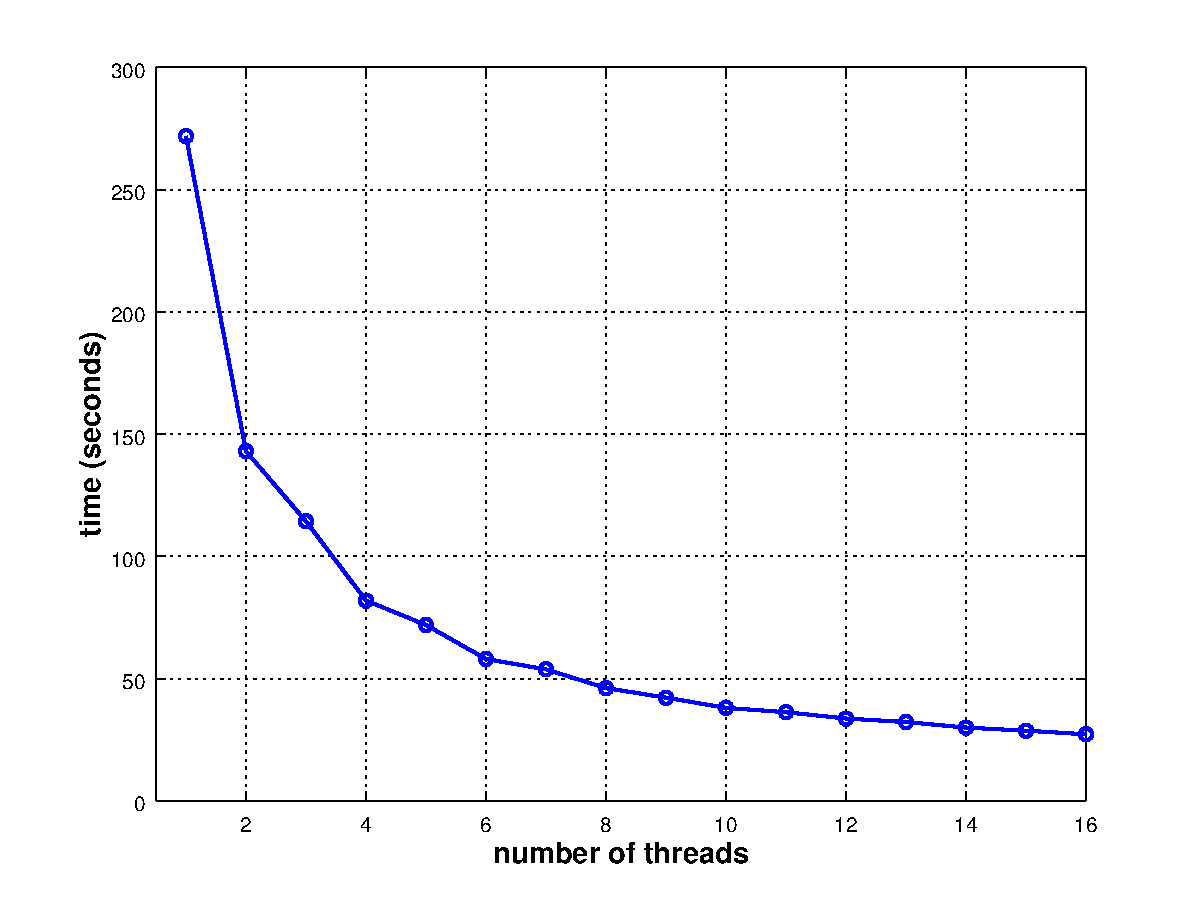
\includegraphics[width=1.1\textwidth]{plot1.pdf}\\
    {(a)}
  \end{minipage}%
  \begin{minipage}{0.5\textwidth}
    \centering
    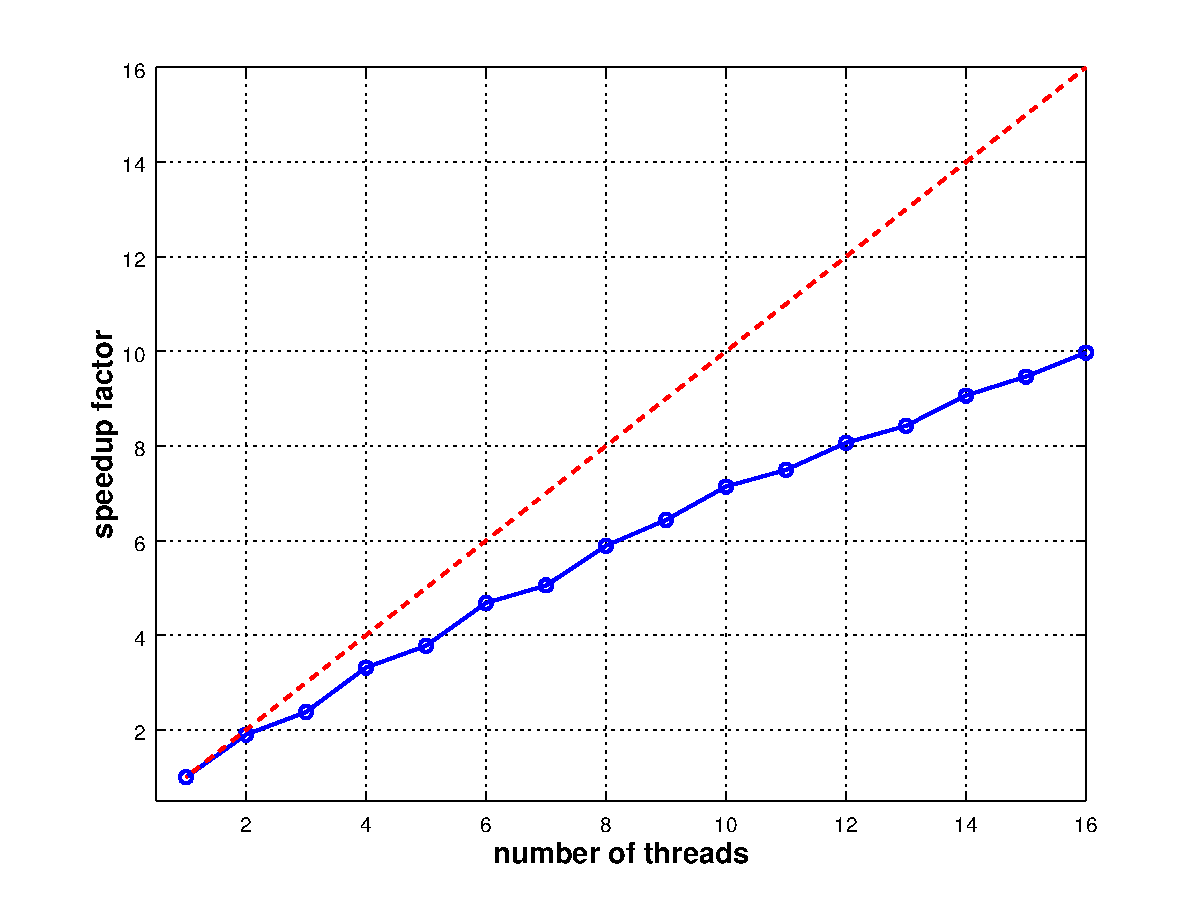
\includegraphics[width=1.1\textwidth]{plot2.pdf}\\
    {(b)}
  \end{minipage}
\end{minipage}
\caption
  {
  Execution characteristics for training a 100 component GMM
  to model a synthetic dataset comprising 1,000,000 samples with 100 dimensions,
  using 10 iterations of the {\it k}-means algorithm and 10 iterations of the EM algorithm:
  {\bf (a)}~total~time~taken depending on the number of threads;
  {\bf (b)}~corresponding speedup factor compared to using one thread (blue line), and idealised linear speedup under the assumption of no overheads and no memory access contention (red dotted line).
  The modelling was done on a machine with dual Intel Xeon E5-2620-v4 CPUs, providing 16 independent processing cores running at 2.1~GHz.
  Compilation was done with the GCC 5.4 C++ compiler with the following configuration options: \texttt{-O3 -march=native -fopenmp}.
  }
\label{fig:speedup}
\end{figure*}


\subsection{Comparison with Full-Covariance GMMs in MLPACK}

% I guess we should move the parallelism experiment here, if you go with this
% approach.

% This paragraph could be reworked---it doesn't really fit with the "flow" of
% the paper.  But I think it would be nice to show that using a diagonal GMM
% doesn't cost us too much---because that would be my primary concern as a
% reviewer (i.e. "this contribution doesn't matter because nobody uses diagonal
% GMMs").
In order to validate our intuition that a diagonal GMM is a good choice instead
of the significantly more complex problem of estimating GMMs with full covariance matrices,
we compare the {\it gmm\_diag} class (described in Section~\ref{sec:implementation})
against the full-covariance GMM implementation in the well-established MLPACK C++ machine learning library~\cite{Curtin_2013}.

We selected common datasets from the UCI machine learning dataset repository~\cite{Lichman_2013},
and trained both diagonal and full-covariance GMMs on these datasets.
The number of Gaussians was chosen according to the original source of each dataset;
where possible, 3 times the number of classes in the dataset was used.
In some cases, small amounts of Gaussian noise was added to the dataset to ensure
training stability of the full-covariance GMMs.
% It takes too long to do BIC on this, we don't have time.  We could handle it
% after reviews possibly?  Really the number of Gaussians does not matter
% anyway, we only care here about how long it takes.
Both implementations used 10 iterations of {\it k}-means for initialisation,
followed by running the EM algorithm until convergence or reaching a maximum of 250 iterations.
The entire fitting procedure was repeated 10 times, each time with a different random starting point.

The results are given in Table \ref{tab:results}, which shows the best log-likelihood of the 10 runs,
the average wall-clock runtime for the fitting,
as well as dataset information
(number of samples, dimensionality, and number of Gaussians used for modelling).
We can see that the diagonal GMM implementation in 
the {\it gmm\_diag} class provides speedups from one to two orders-of-magnitude
over the full-covariance implementation in \mbox{MLPACK}.
% The speedup is more pronounced the more dimensions there are in a dataset.
Furthermore, in most cases there is no significant loss in goodness-of-fit (as measured by log-likelihood).
% In one case ({\it ozone}) the goodness-of-fit is lower; we conjecture that using a larger $N_G$ for the {\it gmm\_diag} class will improve the accuracy of the model.
In several cases ({\it winequality}, {\it phy}, {\it covertype}, {\it pokerhand})
the log-likelihood is notably higher for the {\it gmm\_diag} class;
we conjecture that in these cases the diagonal covariance matrices are acting as a form of regularisation to reduce overfitting~\cite{Bishop_2006}.


\begin{table*}[!tb]
%\vspace{5ex}
\centering
\normalsize
\begin{tabular}{|l|c|c|c|c|c|c|c|c|}
\hline
\multirow{2}{*}{\bfseries dataset} & {\bfseries num.}    & {\bfseries num.} & {\bfseries num.}  & {\bfseries MLPACK}   & {\bfseries {gmm\_diag}} & $\sfrac{\mbox{\bfseries MLPACK}}{\mbox{\bfseries gmm\_diag}}$ & {\bfseries MLPACK}             & {\bfseries {gmm\_diag}}        \\
                                   & {\bfseries samples} & {\bfseries dims} & {\bfseries Gaus.} & {\bfseries fit time} & {\bfseries fit time}    & {\bfseries fit time ratio}                                    & {$\mathbf \log~p(X|\lambda) $} & {$\mathbf \log~p(X|\lambda) $} \\
\hline
  cloud       & {\tt ~~~~2,048} & {\tt 10} & {\tt ~5} & {\tt ~~~~1.50s} &  {\tt\bfseries ~0.14s} & {\tt ~10.7} & {\tt~-59.98{\tiny$\times$}10$^{\mathtt 3}$} & {\tt          ~-64.12{\tiny$\times$}10$^{\mathtt 3}$} \\
  ozone       & {\tt ~~~~2,534} & {\tt 72} & {\tt ~6} & {\tt ~~~~8.59s} &  {\tt\bfseries ~0.10s} & {\tt ~85.9} & {\tt-226.13{\tiny$\times$}10$^{\mathtt 3}$} & {\tt          -307.95{\tiny$\times$}10$^{\mathtt 3}$} \\
  winequality & {\tt ~~~~6,497} & {\tt 11} & {\tt 30} & {\tt ~~~16.10s} &  {\tt\bfseries ~0.68s} & {\tt ~23.7} & {\tt~-47.12{\tiny$\times$}10$^{\mathtt 3}$} & {\tt\bfseries ~-15.85{\tiny$\times$}10$^{\mathtt 3}$} \\
  corel       & {\tt ~~~37,749} & {\tt 32} & {\tt 50} & {\tt ~~544.62s} &  {\tt\bfseries ~4.55s} & {\tt 119.7} & {\tt~~+4.52{\tiny$\times$}10$^{\mathtt 6}$} & {\tt          ~~+4.44{\tiny$\times$}10$^{\mathtt 6}$} \\
  birch3      & {\tt ~~100,000} & {\tt ~2} & {\tt ~6} & {\tt ~~~18.13s} &  {\tt\bfseries ~2.39s} & {\tt ~~7.6} & {\tt~~-2.70{\tiny$\times$}10$^{\mathtt 6}$} & {\tt          ~~-2.71{\tiny$\times$}10$^{\mathtt 6}$} \\
  phy         & {\tt ~~150,000} & {\tt 78} & {\tt 30} & {\tt ~3867.12s} &  {\tt\bfseries 29.25s} & {\tt 132.2} & {\tt~~-2.10{\tiny$\times$}10$^{\mathtt 7}$} & {\tt\bfseries ~~-1.88{\tiny$\times$}10$^{\mathtt 7}$} \\
  covertype   & {\tt ~~581,012} & {\tt 55} & {\tt 21} & {\tt 10360.53s} &  {\tt\bfseries 64.83s} & {\tt 159.8} & {\tt~~-9.46{\tiny$\times$}10$^{\mathtt 7}$} & {\tt\bfseries ~~-6.90{\tiny$\times$}10$^{\mathtt 7}$} \\
  pokerhand   & {\tt 1,000,000} & {\tt 10} & {\tt 25} & {\tt ~3653.94s} &  {\tt\bfseries 55.85s} & {\tt ~65.4} & {\tt~~-1.90{\tiny$\times$}10$^{\mathtt 7}$} & {\tt\bfseries ~~-1.68{\tiny$\times$}10$^{\mathtt 7}$} \\
\hline
\end{tabular}
\vspace{1ex}
\caption
  {
  Comparison of fitting time (seconds) and goodness-of-fit (as measured by log-likelihood) using full covariance GMMs from the MLPACK library~\cite{Curtin_2013}
  against diagonal GMMs in the {\it gmm\_diag} class,
  on common datasets from the UCI machine learning dataset repository~\cite{Lichman_2013}.
  The lower the fitting time, the better.
  The higher the $\log p(X|\lambda)$, the better.
  }
\label{tab:results}
\end{table*}


%% CS: I thought about the data you sent by email (matched results) and a good way to explain the story,
%% CS: but so far I haven'tt come up with something that was easy to grasp and didn't raise more questions.
%% CS: I think the way forward would be to choose a result from Table I (comparison against full cov GMM)
%% CS: where gmm_diag is getting a notably worse log-likelihood for the same N_G as the full cov GMM,
%% CS: and then see if the log-likelihood can be improved by increasing N_G.
%% CS: At that point we can compare the amout of time taken by full cov GMM and gmm_diag with higher N_G.

% Additionally, we perform a more detailed investigation of the behavior of each
% implementation on the {\tt corel} dataset.  In order to verify the results of
% Reynolds~\cite{Reynolds_2000}, we train diagonal and full-covariance GMMs on a
% variety of choices of $N_g$, collecting the log-likelihood of the trained model
% at each EM iteration.  This shows us how quickly each model is able to fit to
% the data.  Figure~\ref{fig:lc} shows the resulting learning curve, demonstrating
% that the diagonal GMM implementation is able to converge to a better
% log-likelihood in less time than the full-covariance implementation.
% 
% \begin{figure*}
% \begin{center}
% % This figure is horrible.  I have not thought of a better way to plot this
% % here.  But maybe it is a start.  Like for real this is the ugliest graph I
% % have ever produced in my life.
% % \includegraphics[width=\textwidth]{data/garbage_fire.png}
% \end{center}
% \caption{GMM training time vs. log-likelihood of model for diagonal GMMs (blue)
% and non-diagonal GMMs (red).  The simulation is performed for many values of
% $N_g$, showing that for the {\tt corel} dataset, we can get a faster and better
% fit with our implementation of diagonal GMMs than with a full-covariance GMM,
% even when the diagonal GMM must have a greater $N_g$ to achieve a better fit.}
% \label{fig:lc}
% \end{figure*}

% done with N_G = 30
% 
% birch     full        -2.5941e6       82.4212s
% birch     gmm_diag    -2.62008e6      8.1022s
% 
% phy       full        -2.36e7         5102.751s
% phy       gmm_diag    -7.94981e6      78.44s
% 
% covertype full        -1.09351e8      13221.844s
% covertype gmm_diag    -5.190e7        344.413s



% \begin{table*}[!tb]
% \vspace{5ex}
% \centering
% \small
% \begin{tabular}{|l|c|c|c|c|c|c|c|}
% \hline
% {\bf Dataset} & {\bf $N_v$} & {\bf dims} & {\bf $N_g$} & {\bf MLPACK fit time} & {\bfseries {\it\bfseries gmm\_diag} fit time} & {\bf MLPACK $\log(p(X|\lambda))$} & {\bf {\it\bfseries gmm\_diag} $\log(p(X|\lambda))$} \\
% \hline
%   cloud       & ~~2,048 & 10 &  5 & ~~~~~1.375s & ~~~{\bf 0.164s} & $-59.9  \times 10^{3}$ & $-63.0  \times 10^{3}$ \\
%   ozone       & ~~2,534 & 72 &  6 & ~~~~~1.982s & ~~~{\bf 0.202s} & $-230   \times 10^{3}$ & $-399   \times 10^{3}$ \\
%   winequality & ~~6,497 & 11 & 30 & ~~~~18.201s & ~~~{\bf 1.257s} & $-47.5  \times 10^{3}$ & $-15.6  \times 10^{3}$ \\
%   corel       & ~37,749 & 32 & 50 & ~~~501.601s &  ~{\bf 22.016s} & $~~2.99 \times 10^{6}$ & $~~2.89 \times 10^{6}$ \\
%   cup98b      & ~95,413 & 56 & 30 &  ~1207.860s &  ~{\bf 48.425s} & $-11.9  \times 10^{6}$ & $-6.62  \times 10^{6}$ \\
% % birch3      & 100,000 & 2  &  6 & \\
%   birch3      & 100,000 & ~2 & 30 & ~~~~82.421s &  ~~{\bf 8.102s} & $-2.59  \times 10^{6}$ & $-2.62  \times 10^{6}$ \\
%   phy         & 150,000 & 78 & 30 &  ~5102.751s &  ~{\bf 78.440s} & $-2.36  \times 10^{7}$ & $-7.94  \times 10^{6}$ \\
% % covertype   & 581,012 & 55 & 21 & \\
%   covertype   & 581,012 & 55 & 30 &  13221.844s &  {\bf 344.413s} & $-1.09  \times 10^{8}$ & $-5.19  \times 10^{7}$ \\
% % pokerhand   & 1000000 & 10 & 25 & 30 & \\
% \hline
% \end{tabular}
% \caption
%   {
%   Comparison of fitting time (seconds) and goodness-of-fit (as measured by log-likelihood) using full covariance GMMs from the MLPACK library~\cite{Curtin_2013}
%   against diagonal GMMs in the {\it gmm\_diag} class,
%   on common datasets from the UCI machine learning dataset repository~\cite{Lichman_2013}.
%   $N_v$ indicates the number of samples, {\it dims} indicates dimensionality, and $N_G$ the number of Gaussians.
%   }
% \label{tab:results}
% \end{table*}

% \begin{table*}
% \begin{center}
% \begin{tabular}{|l|c|c|c|c|c|c|c|}
% \hline
% {\bf dataset} & {\bf $N_v$} & {\bf dims} & {\bf $N_g$} & {\bf full-covariance fit time} & {\bf Armadillo fit time} & {\bf full-diagonal $\log(p(X|\lambda))$} & {\bf Armadillo $\log(p(X|\lambda))$} \\
% \hline
% cloud & 2048 & 10 & 5 & 1.375s & {\bf 0.164s} & -59.9k & -63.0k \\
% ozone & 2534 & 72 & 6 & 1.982s & {\bf 0.202s} & -230k & -399k \\
% winequality & 6497 & 11 & 30 & 18.201s & {\bf 1.257s} & -47.5k & -15.6k
% \\
% corel & 37749 & 32 & 50 & 501.601s & {\bf 22.016s} & 2.99M & 2.89M \\
% cup98b & 95413 & 56 & 30 & 1207.86s & {\bf 48.425s} & -11.9M & -6.62M \\
% birch3 & 100000 & 2 & 6 & \\
% phy & 150000 & 78 & 30 & & {\bf 78.44s} & & -7.94M \\
% covertype & 581012 & 55 & 21 & \\
% pokerhand & 1000000 & 10 & 25 & 30 & \\
% \hline
% \end{tabular}
% \end{center}
% \caption{Datasets used for comparisons with full-covariance GMM estimation.}
% \label{tab:results}
% \end{table*}

% \begin{table*}
% \begin{center}
% \begin{tabular}{|l|c|c|c|c|c|c|c|}
% \hline
% {\bf dataset} & {\bf $N_v$} & {\bf dims} & {\bf $N_g$} & {\bf
% full-covariance fit time} & {\bf Armadillo fit time} & {\bf full-diagonal
% $\log(p(X|\lambda))$} & {\bf Armadillo $\log(p(X|\lambda))$} \\
% \hline
% cloud & 2048 & 10 & 5 & 1.375s & {\bf 0.164s} & -59.9k & -63.0k \\
% ozone & 2534 & 72 & 6 & 1.982s & {\bf 0.202s} & -230k & -399k \\
% winequality & 6497 & 11 & 30 & 18.201s & {\bf 1.257s} & -47.5k & -15.6k \\
% corel & 37749 & 32 & 50 & 501.601s & {\bf 22.016s} & 2.99M & 2.89M \\
% cup98b & 95413 & 56 & 30 & & {\bf 48.425s} &  & -6.62M \\
% birch3 & 100000 & 2 & 6 & \\
% phy & 150000 & 78 & 30 & \\
% covertype & 581012 & 55 & 21 & \\
% pokerhand & 1000000 & 10 & 25 & 30 & \\
% \hline
% \end{tabular}
% \end{center}
% \caption{Datasets used for comparisons with full-covariance GMM estimation.}
% \label{tab:results}
% \end{table*}


\section{Conclusion}

% In this paper we have demonstrated a parallelised implementation of Gaussian
% Mixture Models, which is released as part of the publicly available Armadillo
% C++ linear algebra library.  Through effective parallelization and restriction
% of the problem to diagonal-covariance settings, we show that the Armadillo
% implementation is able to significantly outperform other GMM implementations
% without significant fitting losses.

In this paper we have demonstrated a parallelised (multi-threaded) and robust implementation
of Gaussian Mixture Models in the C++ language.
Parallelisation is achieved through reformulation of the Expectation-Maximisation and {\it k}-means algorithms into a MapReduce-like framework.
The implementation also uses several techniques to improve numerical stability and improve modelling accuracy.
We demonstrated that the implementation achieves a speedup of an order of magnitude on a recent 16 core machine,
and that it can achieve higher modelling accuracy than a well-established publically accessible implementation.
The parallelised implementation is released as open source software
and included in recent releases of the cross-platform Armadillo C++ linear algebra library.
The library is provided under the permissive Apache 2.0 license, allowing unencumbered use in commercial products.
  


%\balance
\renewcommand{\baselinestretch}{1.1}\small\normalsize
\bibliographystyle{ieee}
\bibliography{refs}
\clearpage

% \newpage
% \appendix
% \section*{Appendix A: Abridged Derivation of the EM Algorithm for Gaussian Mixture Models}
\label{app:em_algorithm}

In the Gaussian Mixture Model (GMM) approach, the distribution of samples (vectors) is modelled as:
%
\begin{equation}
	p(\Vec{x} | \Theta) = \sum\nolimits_{m=1}^{M} w_m p(\Vec{x}| \theta_m)
	\label{eqn:mixture_fn}
\end{equation}

\noindent
where $\Vec{x}$ is a $D$-dimensional vector,
$w_m$ is a weight (with constraints $\sum\nolimits_{m=1}^{M} w_m = 1$, $w_m \geq 0$),
and
$p(\Vec{x}| \theta_m)$ is a multivariate Gaussian density function with parameter set $\theta_m = \{ \Vec{\mu}_m, \Mat{\Sigma}_m \}$:
%
\begin{equation}
	p(\Vec{x}| \theta_m) =  {{\mathcal{N}}}( \Vec{x} | \Vec{\mu}_m, \Mat{\Sigma}_m )  = 
		\frac{1}{ (2\pi)^{\frac{D}{2}} | \Mat{\Sigma}_m|^{\frac{1}{2}} }
		\exp \left[ -\frac{1}{2} (\Vec{x}-\Vec{\mu}_m)^T \Mat{\Sigma}_m^{-1} (\Vec{x}-\Vec{\mu}_m) \right]
%
\end{equation}%

\noindent
where $\Vec{\mu}_m$ is the mean vector and $\Mat{\Sigma}_m$ is the covariance matrix.
Thus the complete parameter set for Eqn.~(\ref{eqn:mixture_fn}) is expressed as $\Theta = \{w_m, \theta_m\}_{m=1}^{M}$.
Given a set of training samples, $X=\{\Vec{x}_i\}_{i=1}^{N}$,
we need to find $\Theta$ that suitably models the underlying distribution.
Stated more formally, we need to find $\Theta$ that maximises the following likelihood function:
%
\begin{equation}
	p(X | \Theta) = \prod\nolimits_{i=1}^{N} p(\Vec{x}_i | \Theta)
	\label{eqn:lhood_fn}
\end{equation}

The Expectation-Maximisation (EM) algorithm~\cite{Dempster77, McLachlan-2008, Moon96, Redner84} is an iterative likelihood function optimisation technique,
often used in the pattern recognition and machine learning~\cite{Bishop_2006,Duda01}.
It is a general method for finding the maximum-likelihood estimate of the parameters of an assumed distribution,
when either the training data is incomplete or has missing values, or when the likelihood function can be made analytically tractable
by assuming the existence of (and values for) {\it missing} data.

To apply the EM algorithm to finding $\Theta$, we must first assume that our training data $X$ is incomplete
and assume the existence of missing data $Y = \{y_i\}_{i=1}^{N}$,
where each $y_i$ indicates the mixture component that ``generated'' the corresponding $\Vec{x}_i$.
Thus $y_i \in [1,M] ~ \forall ~ i$ and $y_i = m$ if the $i$-th feature vector ($\Vec{x}_i$) was ``generated'' by the $m$-th component.
If we know the values for $Y$, then Eqn.~(\ref{eqn:lhood_fn}) can be modified to:
%
\begin{equation}
	p(X,Y | \Theta) = \prod\nolimits_{i=1}^{N} w_{y_i} p(\Vec{x}_i| \theta_{y_i})
	\label{eqn:lhood_fn_modified}
\end{equation}

\noindent
As its name suggests, the EM algorithm is comprised of two steps which are iterated: (i)~expectation, followed by (ii)~maximisation.
In the expectation step, the expected value of the complete data log-likelihood, $\log p(X,Y | \Theta)$,
is found with respect to the unknown data $Y = \{y_i\}_{i=1}^{N}$ given training data $X=\{\Vec{x}_i\}_{i=1}^{N}$ and current parameter estimates,
$\Theta^{[k]}$ (where $k$ indicates the iteration number):
%
\begin{equation}
	Q(\Theta, \Theta^{[k]}) = E \left[ \log p(X,Y | \Theta) ~|~ X,\Theta^{[k]} \right]
	\label{eqn:q_fn}
\end{equation}

\noindent
Since $Y$ is a random variable with distribution $p(\mbox{\boldmath $y$}|X,\Theta^{[k]})$, Eqn.~(\ref{eqn:q_fn}) can be written as:
%
\begin{equation}
	Q(\Theta, \Theta^{[k]}) = \int_{\mbox{\boldmath $y$} \in \Upsilon}
								\log p(X,\mbox{\boldmath $y$} | \Theta) ~ p(\mbox{\boldmath $y$}|X,\Theta^{[k]}) ~~ d \mbox{\boldmath $y$}
	\label{eqn:q_fn2}
\end{equation}

\noindent
where \mbox{\boldmath $y$} is an instance of the missing data and $\Upsilon$ is the space of values \mbox{\boldmath $y$} can take on.
The maximisation step then maximises the expectation:
%
\begin{equation}
	\Theta^{[k+1]} = \arg \max_{\Theta} Q(\Theta, \Theta^{[k]})
	\label{eqn:maximize}
\end{equation}

\noindent
The expectation and maximisation steps are iterated until convergence,
or when the increase in likelihood falls below a pre-defined threshold.
As can be seen in Eqn.~(\ref{eqn:q_fn2}), we require $p(\mbox{\boldmath $y$}|X,\Theta^{[k]})$.
We can define it as follows:
%
\begin{equation}
	p(\mbox{\boldmath $y$}|X,\Theta^{[k]}) = \prod\nolimits_{i=1}^{N} p(y_i | \Vec{x}_i, \Theta^{[k]})
\end{equation}

\noindent
Given initial parameters%
%
\footnote{Parameters for $k=0$ can be found via the {\it k}-means algorithm~\cite{Bishop_2006,Duda01,Linde80} (see also Section \ref{sec:param_km}).}
%
~$\Theta^{[k]}$,
we can compute $p(\Vec{x}_i | \theta_m^{[k]})$.
Moreover, we can interpret the mixing weights ($w_m$) as {a-priori} probabilities of each mixture component, ie., $w_m = p(m | \Theta^{[k]})$.
Hence we can apply Bayes' rule~\cite{Duda01} to obtain:
%
\begin{eqnarray}
	p(y_i | \Vec{x}_i, \Theta^{[k]}) & = & \frac{ p(\Vec{x}_i | \theta_{y_i}^{[k]}) p(y_i | \Theta^{[k]}) }{ p(\Vec{x}_i | \Theta^{[k]}) } \\
	~ & = & \frac{ p(\Vec{x}_i | \theta_{y_i}^{[k]}) p(y_i | \Theta^{[k]}) }{ \sum\nolimits_{n=1}^{M} p(\Vec{x}_i | \theta_{n}^{[k]}) p(n | \Theta^{[k]})}
	\label{eqn:p_yi}
\end{eqnarray}

\noindent
Expanding Eqn.~(\ref{eqn:q_fn2}) yields:
%
\begin{eqnarray}
	Q(\Theta, \Theta^{[k]}) & = & \int_{\mbox{\boldmath $y$} \in \Upsilon}
									\log p(X,\mbox{\boldmath $y$} | \Theta) ~ p(\mbox{\boldmath $y$}|X,\Theta^{[k]}) ~~ d \mbox{\boldmath $y$} \\
							~ & = & \sum\nolimits_{\mbox{\boldmath $y$} \in \Upsilon}  \log \prod\nolimits_{i=1}^{N} w_{y_i} p(\Vec{x}_i | \theta_{y_i})  
																		\prod\nolimits_{j=1}^{N} p(y_j | \Vec{x}_j, \Theta^{[k]} ) \\
							~ & = & \sum\nolimits_{y_1=1}^{M} \sum\nolimits_{y_2=1}^{M} \cdots \sum\nolimits_{y_N=1}^{M} 
															\sum\nolimits_{i=1}^{N} \log \left[ w_{y_i} p(\Vec{x}_i | \theta_{y_i}) \right] 
															\prod\nolimits_{j=1}^{N} p(y_j | \Vec{x}_j, \Theta^{[k]} )  \label{eqn:q_fn_expanded}
\end{eqnarray}%

\noindent
It can be shown~\cite{Bilmes98} that Eqn.~(\ref{eqn:q_fn_expanded}) can be simplified to:
%
\begin{eqnarray}
	Q(\Theta, \Theta^{[k]}) & = & \sum\nolimits_{m=1}^{M}  \sum\nolimits_{i=1}^{N} \log[ w_m  p(\Vec{x}_i | \theta_m)] ~ p(m|\Vec{x}_i, \Theta^{[k]}) \\
							~ & = & \sum\nolimits_{m=1}^{M}  \sum\nolimits_{i=1}^{N} \log[ w_m ] ~  p(m|\Vec{x}_i, \Theta^{[k]}) +
									\sum\nolimits_{m=1}^{M}	\sum\nolimits_{i=1}^{N} \log[  p(\Vec{x}_i | \theta_m) ] ~ p(m|\Vec{x}_i, \Theta^{[k]}) ~~~ \\
							~ & = & Q_1 ~~~ + ~~~ Q_2 
\end{eqnarray}%

\noindent
Hence $Q_1$ and $Q_2$ can be maximised separately, to obtain $w_m$ and $\theta_m = \{ \Vec{\mu}_m, \Mat{\Sigma}_m \}$, respectively.
To find the expression which maximises $w_m$, we need to introduce the Lagrange multiplier~\cite{Duda01} $\psi$,
with the constraint $\sum\nolimits_m w_m = 1$, take the derivative of $Q_1$ with respect to $w_m$ and set the result to zero:
%
\begin{eqnarray}
	\frac{\partial Q_1}{\partial w_m} & = & 0 \\
						\therefore ~ 0  & = & \frac{\partial}{\partial w_m}
											\left\{ \sum\nolimits_{m=1}^{M} \sum\nolimits_{i=1}^{N} \log[ w_m ]  ~ p(m|\Vec{x}_i, \Theta^{[k]})
											 		+ \psi \left[ (\sum\nolimits_m w_m) -1 \right] \right\} \\
									~ & = & \sum\nolimits_{i=1}^{N} \frac{1}{w_m} ~ p(m|\Vec{x}_i, \Theta^{[k]}) + \psi \label{eqn:q1_alpha_opt}
\end{eqnarray}

\noindent
Rearranging Eqn.~(\ref{eqn:q1_alpha_opt}) to obtain a value for $\psi$:
%
\begin{eqnarray}
	-\psi w_m & = & \sum\nolimits_{i=1}^{N} p(m|\Vec{x}_i, \Theta^{[k]})
\end{eqnarray}

\noindent
Summing both sides over $m$ yields:
%
\begin{eqnarray}
	-\psi \sum\nolimits_m w_m & = & \sum\nolimits_{i=1}^{N} \sum\nolimits_m p(m|\Vec{x}_i, \Theta^{[k]}) \\
	-\psi 1 & = & \sum\nolimits_{i=1}^{N} 1 \\
	\psi & =  & -N	\label{eqn:lambda_equals_negN}
\end{eqnarray}

\noindent
By substituting Eqn.~(\ref{eqn:lambda_equals_negN}) into Eqn.~(\ref{eqn:q1_alpha_opt}) we obtain:
%
\begin{eqnarray}
			N & = & \sum\nolimits_{i=1}^{N} \frac{1}{w_m} ~ p(m|\Vec{x}_i, \Theta^{[k]}) \\
	\therefore ~ w_m & = & \frac{1}{N} \sum\nolimits_{i=1}^{N} p(m|\Vec{x}_i, \Theta^{[k]}) 
	\label{eqn:alpha_m_solved}
\end{eqnarray}

\noindent
To find expressions which maximise $\Vec{\mu}_m$ and $\Mat{\Sigma}_m$, let us now expand $Q_2$:
%
\begin{eqnarray}
	Q_2 & = &   \sum\nolimits_{m=1}^{M}	\sum\nolimits_{i=1}^{N} \log[  p(\Vec{x}_i | \theta_m) ] ~ p(m|\Vec{x}_i, \Theta^{[k]}) 	\\
	 ~  & = &   \sum\nolimits_{m=1}^{M} \sum\nolimits_{i=1}^{N} \left[
					- \frac{1}{2} \log(|\Mat{\Sigma}_m|) - \frac{1}{2} (\Vec{x}_i - \Vec{\mu}_m)^T \Mat{\Sigma}_m^{-1} (\Vec{x}_i - \Vec{\mu}_m)
					\right] p(m|\Vec{x}_i, \Theta^{[k]})  \label{eqn:q2_expanded}
\end{eqnarray}

\noindent
where $-\frac{D}{2} \log(2\pi)$ was omitted since it vanishes when taking a derivative with respect to $\Vec{\mu}_m$ or $\Mat{\Sigma}^{-1}_m$.
To find the expression which maximises $\Vec{\mu}_m$, we need to take the derivative of $Q_2$ with respect to $\Vec{\mu}_m$, and set the result to zero:
%
\begin{eqnarray}
	\frac{\partial Q_2}{\partial \Vec{\mu}_m} & = & 0   \\
 0 & = & \frac{\partial}{\partial \Vec{\mu}_m} \left\{ \sum\nolimits_{m=1}^{M} \sum\nolimits_{i=1}^{N} \left[
					- \frac{1}{2} \log(|\Sigma_m|) - \frac{1}{2} (\Vec{x}_i - \Vec{\mu}_m)^T \Mat{\Sigma}_m^{-1} (\Vec{x}_i - \Vec{\mu}_m)
					\right] p(m|\Vec{x}_i, \Theta^{[k]}) \right\} ~~~ ~~~ ~~~  \label{eqn:q2_mu_partone}
\end{eqnarray}%

\noindent
L\"{u}tkepohl~\cite{Lutkepohl96} states that
\mbox{$\frac{ \partial \Vec{z}^T \Mat{A} \Vec{z} }{ \partial \Vec{z} } =  (\Mat{A} + \Mat{A}^T)\Vec{z}$},
~ $(\Mat{A}^{-1})^T = (\Mat{A}^T)^{-1}$ and if $\Mat{A}$ is symmetric, then $\Mat{A} = \Mat{A}^T$.
Since $\Mat{\Sigma}_m$ is symmetric, Eqn.~(\ref{eqn:q2_mu_partone}) reduces to:
%
\begin{eqnarray}
	0 & = & \sum\nolimits_{i=1}^{N} - \frac{1}{2} 2 \Mat{\Sigma}_m^{-1} (\Vec{x}_i - \Vec{\mu}_m) p(m|\Vec{x}_i, \Theta^{[k]}) \\
	~ & = & \sum\nolimits_{i=1}^{N} \left[ - \Mat{\Sigma}_m^{-1} \Vec{x}_i p(m|\Vec{x}_i, \Theta^{[k]}) + \Mat{\Sigma}_m^{-1} \Vec{\mu}_m p(m|\Vec{x}_i, \Theta^{[k]})  \right] ~~~ \\
	\therefore ~ \sum\nolimits_{i=1}^{N} \Mat{\Sigma}_m^{-1} \Vec{\mu}_m p(m|\Vec{x}_i, \Theta^{[k]}) & = & \sum\nolimits_{i=1}^{N} \Mat{\Sigma}_m^{-1} \Vec{x}_i p(m|\Vec{x}_i, \Theta^{[k]}) 
\end{eqnarray}%

\noindent
Multiplying both sides by $\Mat{\Sigma}_m$ yields:
%
\begin{eqnarray}
	\sum\nolimits_{i=1}^{N} \Vec{\mu}_m p(m|\Vec{x}_i, \Theta^{[k]}) & = & \sum\nolimits_{i=1}^{N} \Vec{x}_i p(m|\Vec{x}_i, \Theta^{[k]})  \\
\therefore ~ \Vec{\mu}_m & = & \frac{ \sum\nolimits_{i=1}^{N} \Vec{x}_i p(m|\Vec{x}_i, \Theta^{[k]}) }
								   { \sum\nolimits_{i=1}^{N} p(m|\Vec{x}_i, \Theta^{[k]}) }
\end{eqnarray}

\noindent
L\"{u}tkepohl~\cite{Lutkepohl96} states that:  
$|\Mat{A}^{-1}| = |\Mat{A}|^{-1}$ 
and 
$\mbox{tr}(\Mat{A}\Mat{B}) = \mbox{tr}(\Mat{B}\Mat{A})$.
Since $\mbox{tr}{(\Vec{z}A\Vec{z}^T)} = \mbox{tr}(\mbox{scalar})$,
we can rewrite Eqn.~(\ref{eqn:q2_expanded}) as:
%
\begin{eqnarray}
	Q_2 & = &   \sum\nolimits_{m=1}^{M} \sum\nolimits_{i=1}^{N} \left[
					\frac{1}{2} \log(|\Mat{\Sigma}_m^{-1}|) - \frac{1}{2} \mbox{tr}(\Mat{\Sigma}_m^{-1} (\Vec{x}_i - \Vec{\mu}_m) (\Vec{x}_i - \Vec{\mu}_m)^T)
					\right] p(m|\Vec{x}_i, \Theta^{[k]})  \label{eqn:q2_rewritten}
\end{eqnarray}

\noindent
According to L\"{u}tkepohl~\cite{Lutkepohl96},
$\frac{\partial \log(|\Mat{A}|)}{\partial \Mat{A}} = (\Mat{A}^{T})^{-1}$
and $\frac{\partial \mbox{tr}(\Mat{B}\Mat{A})}{\partial \Mat{B}} = \Mat{A}^T$.
Moreover, we note that $\Vec{z}\Vec{z}^T$ is a symmetric matrix.
To find an expression which maximises~$\Mat{\Sigma}_m$,
we can take the derivative of Eqn.~(\ref{eqn:q2_rewritten}) with respect to $\Mat{\Sigma}_m^{-1}$
and set the result to zero:
%
\begin{eqnarray}
	0 & = & \frac{\partial Q_2}{\partial \Mat{\Sigma}_m^{-1}}  \\
	~ & = & \frac{\partial}{\partial  \Mat{\Sigma}_m^{-1}} \left\{
		\sum\nolimits_{m=1}^{M} \sum\nolimits_{i=1}^{N} \left[
					\frac{1}{2} \log(|\Mat{\Sigma}_m^{-1}|) - \frac{1}{2} \mbox{tr}\left(\Mat{\Sigma}_m^{-1} (\Vec{x}_i - \Vec{\mu}_m) (\Vec{x}_i - \Vec{\mu}_m)^T \right)
					\right] p(m|\Vec{x}_i, \Theta^{[k]})
	\right\} \\
	~ & = & \sum\nolimits_{i=1}^{N} \left[ \frac{1}{2} \Mat{\Sigma}_m - \frac{1}{2} (\Vec{x}_i - \Vec{\mu}_m) (\Vec{x}_i - \Vec{\mu}_m)^T \right] p(m|\Vec{x}_i, \Theta^{[k]}) \\
\end{eqnarray}%

\noindent
thus
%
\begin{eqnarray}
	\frac{1}{2} \Mat{\Sigma}_m \sum\nolimits_{i=1}^{N} p(m|\Vec{x}_i, \Theta^{[k]}) & = & \frac{1}{2} \sum\nolimits_{i=1}^{N} 
																		(\Vec{x}_i - \Vec{\mu}_m) (\Vec{x}_i - \Vec{\mu}_m)^T p(m|\Vec{x}_i, \Theta^{[k]}) \\
	\therefore ~ \Mat{\Sigma}_m & = & \frac{\sum\nolimits_{i=1}^{N} (\Vec{x}_i - \Vec{\mu}_m) (\Vec{x}_i - \Vec{\mu}_m)^T p(m|\Vec{x}_i, \Theta^{[k]})}
						{\sum\nolimits_{i=1}^{N} p(m|\Vec{x}_i, \Theta^{[k]})}
\end{eqnarray}
%\end{small}

\noindent
In summary,
%
\begin{eqnarray}
	w_m^{[k+1]}	& = & \frac{1}{N} \sum\nolimits_{i=1}^{N} p(m|\Vec{x}_i, \Theta^{[k]})  \label{eqn:copy_of_solved_alpha}  \\  
	\Vec{\mu}_m^{[k+1]} & = & \frac{ \sum\nolimits_{i=1}^{N} \Vec{x}_i ~ p(m|\Vec{x}_i, \Theta^{[k]}) }
								   { \sum\nolimits_{i=1}^{N} p(m|\Vec{x}_i, \Theta^{[k]}) }  \label{eqn:copy_of_solved_mu} \\
	\Mat{\Sigma}_m^{[k+1]}	& = & \frac{\sum\nolimits_{i=1}^{N} (\Vec{x}_i - \Vec{\mu}_m^{[k+1]}) (\Vec{x}_i - \Vec{\mu}_m^{[k+1]})^T p(m|\Vec{x}_i, \Theta^{[k]})}
						{\sum\nolimits_{i=1}^{N} p(m|\Vec{x}_i, \Theta^{[k]})}  \label{eqn:copy_of_solved_sigma}
\end{eqnarray}

\noindent
where
%
\begin{equation}
	p(m | \Vec{x}_i, \Theta^{[k]}) = \frac{ p(\Vec{x}_i | \theta_{m}^{[k]}) p(m | \Theta^{[k]}) }{ \sum\nolimits_{n=1}^{M} p(\Vec{x}_i | \theta_{n}^{[k]}) p(n | \Theta^{[k]})}
\end{equation}
%
which can be explicitly stated as:
%
\begin{equation}
	p(m | \Vec{x}_i, \Theta^{[k]}) = \frac{ {\mathcal{N}}( \Vec{x}_i | \Vec{\mu}_m^{[k]},  \Mat{\Sigma}_m^{[k]} )  w_m^{[k]} }
										{ \sum\nolimits_{n=1}^{M} {\mathcal{N}}( \Vec{x}_i | \Vec{\mu}_n^{[k]}, \Mat{\Sigma}_n^{[k]} ) w_n^{[k]} }
\end{equation}

\noindent
If we let $l_{m,i} = p(m | \Vec{x}_i, \Theta^{[k]})$ and $L_m = \sum\nolimits_{i=1}^{N} l_{m,i} $, we can restate Eqns.~(\ref{eqn:copy_of_solved_alpha})
to~(\ref{eqn:copy_of_solved_sigma}) as:
%
\begin{eqnarray}
	w_m^{[k+1]}	& = & \frac{L_m}{N} \\  
	\Vec{\mu}_m^{[k+1]} & = & \frac{1}{L_m} \sum\nolimits_{i=1}^{N} \Vec{x}_i ~ l_{m,i} \\
	\Mat{\Sigma}_m^{[k+1]}	& = & \frac{1}{L_m} \sum\nolimits_{i=1}^{N} (\Vec{x}_i - \Vec{\mu}_m^{[k+1]}) (\Vec{x}_i - \Vec{\mu}_m^{[k+1]})^T  l_{m,i}
\end{eqnarray}



\end{document}
